\documentclass[bachelor, och, referat]{template}

\usepackage[utf8]{inputenc}
\usepackage{graphicx}

\usepackage{pdfpages}
\usepackage{amsmath}

\usepackage[sort,compress]{cite}
\usepackage{amsmath}
\usepackage{amssymb}
\usepackage{amsthm}
\usepackage{fancyvrb}
\usepackage{longtable}
\usepackage{array}
\usepackage[english,russian]{babel}
\usepackage{minted}

\usepackage{tempora}

\usepackage[justification=centering]{caption}
\usepackage[colorlinks=false, hidelinks=true]{hyperref}


\newcommand{\eqdef}{\stackrel {\rm def}{=}}


\begin{document}

\title{Нейронные иммунные сети}

\course{5}

\group{531}

\napravlenie{10.05.01 "--- Компьютерная безопасность}


\author{Токарева Никиты Сергеевича}


\satitle{доцент}
\saname{И.\,И.\, Слеповичев}


\date{2023}

\maketitle

% Включение нумерации рисунков, формул и таблиц по разделам
% (по умолчанию - нумерация сквозная)
% (допускается оба вида нумерации)
%\secNumbering


\tableofcontents

\intro
С развитием области компьютерных наук и техники общество столкнулось с 
возрастающей проблемой киберпреступности. Одним из аспектов этой проблемы 
является разработка и распространение вредоносных программ, известных как 
компьютерные вирусы. В настоящее время обеспечение защиты компьютерных 
систем от подобных вредоносных программ является приоритетным направлением 
в области обеспечения информационной безопасности. Традиционные методы, 
основанные на сигнатурном поиске для выявления компьютерных вирусов, 
эффективны в обнаружении известных угроз, но оказываются неэффективными 
при обнаружении неизвестных вредоносных программ. Время, проходящее с 
момента появления нового компьютерного вируса до его обнаружения 
специалистами антивирусной индустрии, может быть значительным, 
что позволяет современным вредоносным программам распространяться 
и причинять серьезные ущербы. Компьютерные системы с устаревшими 
антивирусными базами становятся беспомощными перед новыми угрозами. 
Эвристические анализаторы, используемые для обнаружения неизвестных 
компьютерных вирусов, на текущий момент далеки от идеальных и часто 
либо ложно классифицируют чистые, неинфицированные файлы как вредоносные 
программы, либо не распознают зловредные программы.

Данная работа представляет собой обзор нейронных иммунных сетей (НИС), в 
которых комбинируются искусственные иммунные системы (ИИС) и самоорганизующиеся 
нейронные сети Т. Кохонена. В рамках исследования рассматривается один из видов самоорганизующихся
нейронных сетей, который применяется в нейронных иммунных сетях, взаимосвязь между биологической 
иммунной системой и искусственными иммунными системами, а также представлены 
алгоритмы, разработанные для обнаружения вирусов с использованием ИИС.

\section{Самоорганизующиеся нейронные сети Кохонена}

Самоорганизующиеся нейронные сети (self-organising neural networks)
характеризуются обучением без учителя, в результате которого происходит 
адаптация сети к решаемой задаче. Их разработал в 80-е гг. XX в.
финский ученый Т. Кохонен. Нейронные сети
Кохонена осуществляют топологическое упорядочивание входного
пространства образов, поступающих на сеть. Они широко применяются
в задачах распознавания и визуализации образов, оптимизации и
управления.

\subsection{Общая характеристика сетей Кохонена}

Данные сети осуществляют отображение $F$ входного $n$-мерного пространства 
образов в выходное $m$-мерное пространство, т. е. $F : R^n \rightarrow R^m$.
При этом обучение здесь происходит без учителя на основе образов,
поступающих на сеть. Если сеть осуществляет кластеризацию данных,
то $m$ характеризует количество кластеров, на которые разбивается входное 
пространство образов. Архитектура нейронной сети в общем случае
представляет собой двуслойную нейронную сеть с прямыми связями (рис. \ref{nn1}).

\begin{figure}[H]
    \centering
    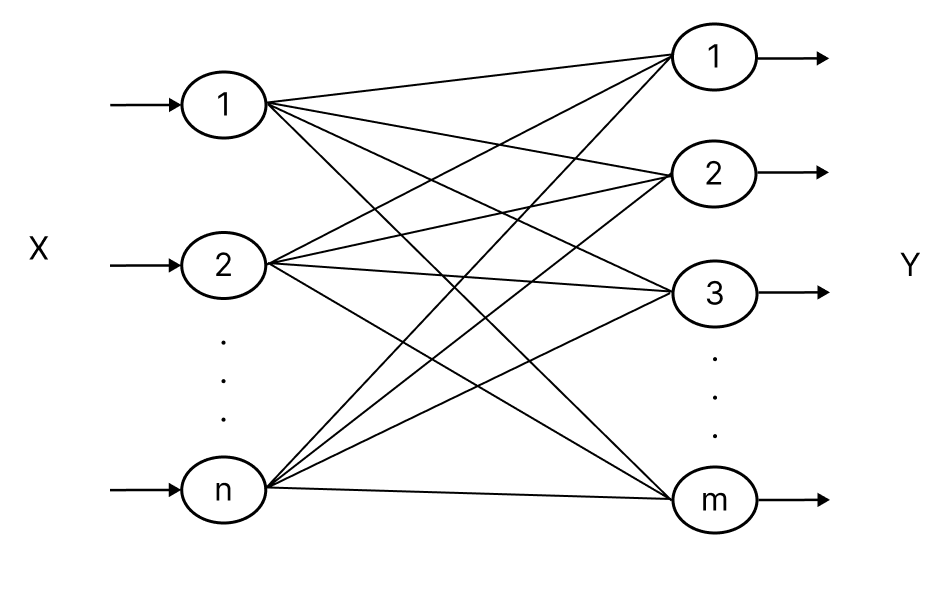
\includegraphics[width=0.7\textwidth]{pics/nn1.png}
    \caption{Архитектура нейронной сети Кохонена}
    \label{nn1}
\end{figure}

Первый слой выполняет чисто распределительные функции, при-
чем каждый нейрон его имеет соединения со всеми нейронными эле-
ментами выходного слоя. Второй слой нейронных элементов является
обрабатывающим.

Нейронная сеть Кохонена использует конкурентный принцип обучения 
и функционирования. В соответствии с этим принципом при подаче 
на сеть входного образа значение только одного нейронного элемента 
выходного слоя принимается равным 1, а выходные значения остальных 
нейронов -- 0. Нейронный элемент, имеющий выходное значение 1, 
называется победителем в конкурентной борьбе. По мере поступления 
входных образов на такую сеть посредством обучения происходит 
разбиение $n$-мерного входного пространства на различные области 
решений, каждой из которых соответствует отдельный нейрон 
обрабатывающего слоя.

Таким образом, самоорганизация таких сетей происходит в результате 
топологического упорядочивания входной информации по различным
зонам, количество которых равно $m$. Такие зоны или области решений
называются кластерами. Топологическое упорядочивание информации
напоминает процессы, происходящие в головном мозге при его развитии, 
когда осуществляется формирование топологически упорядоченных
нейронных структур.

\subsection{Обучающийся векторный квантователь (LVQ)}

Нейронная сеть для векторного квантования была предложена в
1982 г. Т. Кохоненом. Векторное квантование используется для
сжатия данных и основано на идее сопоставления входного вектора с
эталоном. Пусть имеется предварительно сформированное множество 
эталонных данных, каждое из которых называется кодовым вектором. 
Совокупность кодовых векторов называется кодовой книгой. При
поступлении входного вектора происходит его сравнение с вектором из
кодовой книги. В процессе этого выбирается такой кодовый вектор,
который наилучшим образом аппроксимирует входной вектор и его
номер применяется в качестве кода. В качестве меры подобия
между входным и эталонными векторами может использоваться евклидово 
расстояние, а в качестве векторного квантователя -- нейронная
сеть Кохонена. Тогда целью обучения сети является такая настройка
весовых коэффициентов нейрона, которая минимизирует погрешность
аппроксимации между входными образами, создающими $k$-й кластер и
весовыми коэффициентами $k$-го нейрона:

\begin{center}
    $E_k = \frac{1}{2} \sum_{l = 1}^{L_k} \sum_{i = 1}^{n} (x_i^l - w_{ik})^2$,
\end{center}

где $E_k$ -- ошибка квантования для $k$-го кластера.

Общая ошибка квантования определяется как:

\begin{center}
    $E = \sum_{k = 1}^{m} E_k$.
\end{center}

Нейронную сеть для векторного квантования принято называть
обучающимся векторным квантователем (learning vector quantization).
Она представляет собой двуслойную сеть с прямыми связями, как было
показано на рисунке \ref{nn1}. В процессе поступления эталонных векторов на
сеть она обучается так, что образуются кластеры различных эталонов,
каждому из которых соответствует свой нейрон. При поступлении на
вход такой нейронной сети неизвестного образа он идентифицируется
в соответствии с мерой близости к эталонным векторам и кодируется на
выходе сети номером нейрона. Существует большое количество вариантов 
обучения векторного квантователя, однако в данной работе рассмотрены такие
варианты, которые можно использовать в нейронных иммунных сетях.


\subsubsection{Конкурентное обучение с одним победителем}

Здесь в отдельный квант времени только один нейрон может быть
победителем. Процедура обучения векторного квантователя состоит из
следующих шагов:

\begin{enumerate}
    \item Случайно инициализируются весовые коэффициенты нейронной
    сети в диапазоне [0,1].
    \item Задается начальное значение момента времени $t = 0$.
    \item Входные образы последовательно подаются на нейронную сеть
    $x^l, l = 1, L$, и для каждого образа производятся вычисления:
    \begin{enumerate}
        \item[а)] вычисляется евклидово расстояние между входным образом и ве-
        совыми векторами нейронов выходного слоя:

        \begin{center}
            $D_j = |X - W_j| = \sqrt{(x_1 - w_{1j})^2 + (x_1 - w_{2j})^2 + \dots + (x_n - w_{nj})^2}$,
        \end{center}
        где $j = \overline{1, m}$;
        \item[б)] определяется нейрон-победитель, обеспечивающий минималь-
        ное расстояние:
        \begin{center}
            $D_k = \min_j D_j$;
        \end{center}
        \item[в)] производится модификация весовых коэффициентов нейронного
        элемента победителя, а весовые коэффициенты остальных нейронов не
        изменяются:

        \begin{center}
            $w_{ij}(t + 1) = w_{ij}(t) + \gamma(t)(x_i - w{ij}(t)), \text{ если } j = k$,
            $w_{ij}(t + 1) = w_{ij}(t), \text{ если } j \neq k$,
        \end{center}
        где $i = \overline{1, n}, j = \overline{1, m}$.
    \end{enumerate}
    \item Изменяется значение времени $t = t + 1$ и процесс повторяется, 
    начиная с шага 3.
\end{enumerate}

Обучение производится до получения желаемой степени согласования 
между входными и весовыми векторами или до тех пор, пока не
перестанут изменяться весовые коэффициенты. Для остановки процесса 
обучения можно использовать следующие правила:

\begin{enumerate}
    \item[а)] чтобы весовые коэффициенты в процессе обучения перестали
    изменяться, шаг обучения $\gamma(t)$ должен уменьшаться с течением времени, 
    например, по следующему закону:

    \begin{center}
        $\gamma(t) = \gamma_0 e^{-\frac{t}{c}}$,
    \end{center}
    где $\gamma_0 = 0.1$; $c = 1000$;
    \item обычно, как показывает практика, рекомендуется выбирать 
    общее количество эпох обучения $t = (50 \div 200)$.
\end{enumerate}

\subsubsection{Конкурентное обучение со многими победителями}

Для того чтобы похожие кластеры отображались на соседние нейроны 
второго слоя, можно использовать конкурентное обучение со многими 
победителями. В этом случае вокруг нейрона-победителя формируются 
соседние нейроны, для которых также производится модификация
весовых коэффициентов. Для этого вводится специальная функция притяжения, 
определяющая область притяжения нейрона-победителя в конкурентной борьбе. 
Значение функции притяжения для $p$-го нейронного
элемента, не являющегося победителем в конкурентной борьбе, можно
определить в соответствии с функцией Гаусса:

\begin{center}
    $h(t, k, p) = e^{\frac{-|k - p|^2}{2\sigma^2(t)}}$,
\end{center}

где $p$ -- номер нейронного элемента, для которого определяется 
значение функции притяжения; $k$ -- номер нейронного элемента 
победителя; $\sigma(t)$ -- среднеквадратичное отклонение (радиус 
области притяжения), уменьшающееся с течением времени по следующему закону:

\begin{center}
    $\sigma(t) = \sigma_0 e^{-\frac{t}{c}}$.
\end{center}

Значения переменных в последнем выражении можно выбирать следующим образом:

\begin{center}
    $c = \frac{1000}{\log_2{\sigma_0}}$,
\end{center}
где $\sigma_0 = m / 2$.

Тогда модификация весовых коэффициентов производится для всех
нейронных элементов обрабатывающего слоя в соответствии со 
значением функции притяжения:

\begin{center}
    $w_{ip}(t + 1) = w_{ip}(t) + \gamma h(t, k, p)(x_i - w_{ip})$.
\end{center}

В дискретном варианте вводится область притяжения $G$, которая
определяет нейронные элементы, принадлежащие классу победителей.
В этом случае весовые коэффициенты изменяются для всех нейронов,
принадлежащих области $G$:

\begin{equation*}
    \delta w_{ip} = 
    \begin{cases}
        \gamma(t)(x_i - w_{ip}), \text{ если } p \in G, \\
        0, p \notin G. \\
    \end{cases}
\end{equation*}


\section{Искусственные иммунные системы} 
\subsection{Связь биологической иммунной системы с искусственными иммунными системами}

Механизмы, использующиеся в ис­кусственных иммунных системах, позволяют обнаруживать неизвестные
компьютерные вирусы. Искусственные иммунные системы (ИИС) 
базируются на основных принципах биологической иммунной системы (БИС) \cite{ais1}.

БИС является уникальной системой, которая ежедневно борется с болез­нетворными 
бактериями и вирусами, защищая организм от инфекций.
Уникальность БИС заключается в том, что она способна обнаруживать не
только известные вирусы и бактерии, но также и неизвестные. Иммунитет
основан на способности лимфоцитов распознавать собственные клетки
организма от чужеродных клеток.

Основными элементами иммунной системы являются лимфоциты – белые клетки.
Существуют две разновидности лимфоцитов, которые образуются из стволовых клеток в
костном мозге. После синтеза лимфоциты попадают в кровяное русло. Некоторые из них
направляются к тимусу (вилочковой железе), где происходит их созревание (Т-лимфоциты). 
Другие же попадают в лимфатические узлы, и их созревание происходит
там (В-лимфоциты). Процесс созревания незрелых лимфоцитов играет большую роль в
иммунной системе и называется селекцией антител. В результате селекции уничтожаются 
нежелательные для организма лимфоциты. Зрелые лимфоциты имеют на своей поверхности 
детекторы, которые способны обнаруживать специфический антиген (вредные
бактерии, вирусы). Контакт В-клеточных рецепторов со специфическим антигеном и 
связывание определенного его количества стимулируют рост этих клеток и последующее 
многократное деление. В результате образуются многочисленные клетки двух разновидностей:
плазматические и «клетки памяти». Плазматические клетки синтезируют антитела, тем самым 
увеличивая количество клеток, способных обнаруживать вирус. Клетки памяти являются 
копиями В-клеток, однако имеют гораздо больший период жизни, что обеспечивает
защиту организма от повторного заражения вирусом. При связывании определенного
количества вируса, Т-клетки секретируют особую группу веществ, называемую лимфокинами. 
Некоторые лимфокины способны сами разрушать антиген и зараженные клетки.
Другие лимфокины способствуют делению Т-клеток, в результате чего появляется
большое количество антител, способные реагировать на обнаруженный антиген.

\subsection{Описание принципов функционирования ИИС}

Биологическая иммунная система имеет ряд мощных вычислительных возможностей, 
такие как: распознавание, разнообразие, обучение, память, распределенный поиск,
саморегуляция, децентрализация, вероятностное обнаружение.

Построенная по основным принципам биологической иммунной системы, 
искусственная иммунная система обладает всеми ее возможностями
и, на наш взгляд, является перспективной для построения современной
системы компьютерной безопасности для защиты от вредоносных про­грамм. 
ИИС состоит из следующих процессов: создание детекторов, обу­чение и отбор 
детекторов, уничтожение нежелательных детекторов, цир­куляция 
иммунных детекторов в компьютерной системе, уничтожение
детекторов по истечении времени, обнаружение вредоносной программы,
клонирование и мутация детекторов, формирование иммунной памяти. 
Взаимодействие процессов представлено на рисунке \ref{s1}. Все 
перечислен­ные процессы находятся в тесном взаимодействии. Еще одной 
отличи­тельной способностью ИИС является отсутствие единого центра 
управле­ния.

\begin{figure}[H]
    \centering
    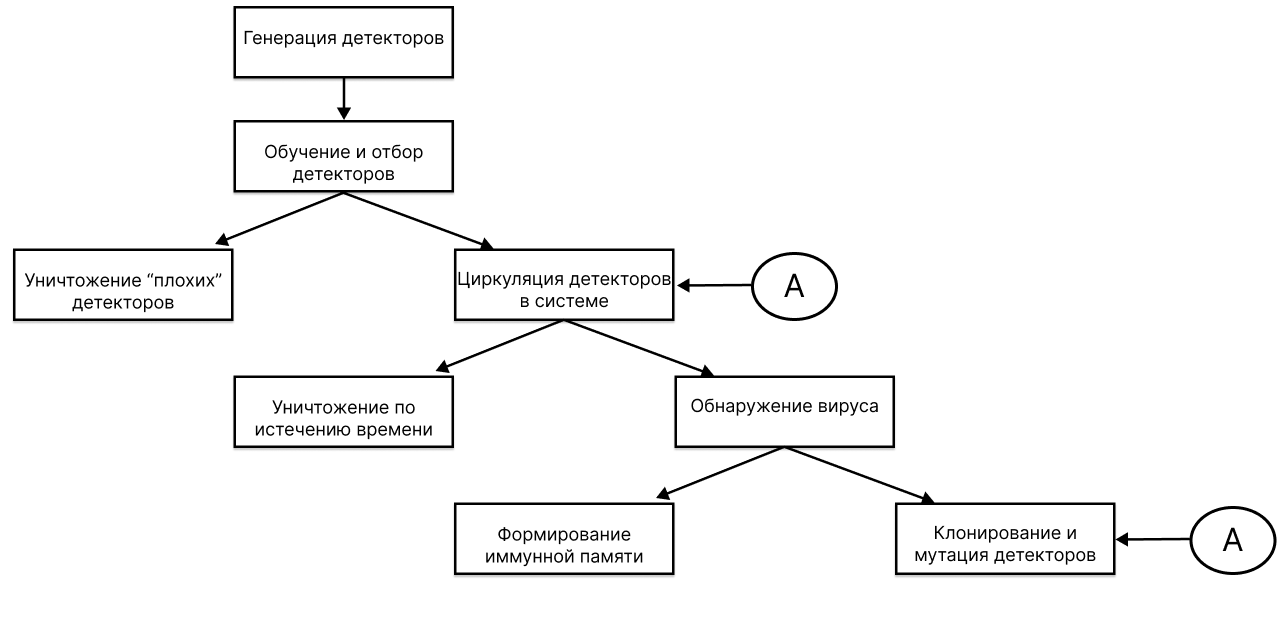
\includegraphics[width=0.7\textwidth]{pics/1.png}
    \caption{Взаимодействие процессов искусственной иммунной системы}
    \label{s1}
\end{figure} 

Рассмотрим подробнее каждый из перечисленных процессов.
Процесс генерации детекторов предназначен для создания иммунных
детекторов, которые являются основными элементами ИИС и выполняют
функцию обнаружения вредоносных программ. Для построения иммун­ных 
детекторов используются искусственные нейронные сети, а именно, 
LVQ сеть (обучающийся векторный квантователь). В процессе ге­нерации 
формируется определенное количество детекторов, каждый из
которых представляет отдельную нейронную сеть.

Первоначально детекторы не способны отличать чистые файлы от вре­доносных 
программ. Поэтому необходим процесс обучения иммунных
детекторов. На стадии обучения иммунные детекторы обучаются распознавать 
зловредные программы и не реагировать на чистые файлы. Обу­чение 
детекторов проходит по следующему алгоритму:

\begin{itemize}
    \item случайным образом выбирается некоторое количество чистых фай­лов 
    (например, утилиты операционной системы) и некоторое количество
    вредоносных программ;
    \item из выбранных файлов также случайным образом выбирается не­
    сколько фрагментов определенной длины (размерность фрагментов зави­сит 
    от количества входов искусственной нейронной сети, которая форми­рует 
    детектор);
    \item выбранные фрагменты образуют обучающую выборку для ИНС и
    подаются на ее вход.
\end{itemize}

Использование разнообразных файлов и вредоносных программ для
формирования обучающей выборки позволяет создавать разнообразные
иммунные детекторы, способные обнаружить вероятные вредоносные
программы.

После обучения детекторы проходят стадию отбора. Механизм отбора
необходим для предотвращения попаданию в компьютерную систему 
не­желательных детекторов. Нежелательным детектором называется такой
детектор, который реагирует на чистые файлы. Такой детектор должен
быть уничтожен.

Обученные иммунные детекторы циркулируют в компьютерной сис­теме, 
проверяя и классифицируя файлы. Каждому детектору отводится
определенное время, на протяжении которого он может находиться в
компьютерной системе. После истечения выделенного времени детектор,
который не обнаружил вредоносной программы, уничтожается, а на его
место приходит новый детектор. Механизм выделения времени для 
существования детектора и уничтожения по истечении выделенного времени
позволяет ИИС избавляться от слабых иммунных детекторов и поддержи­вает 
принцип постоянного обновления детекторов.

При обнаружении иммунным детектором вредоносной программы
происходит процесс клонирования. Клонирование подразумевает созда­ние 
большого количества однотипных детекторов (клонируется тот детек­тор, 
который обнаружил вредоносную программу). Зачастую, при попа­дании 
компьютерного вируса в систему, он заражает большое количество
файлов, путем внедрения копии своего тела в файлы-жертвы. Процесс
клонирования позволяет иммунной системе в кратчайшие сроки изба­виться 
от всех проявлений обнаруженного компьютерного вируса.

После избавления компьютерной системы от вредоносной программы
выбирается наиболее приспособленный к обнаруженному вирусу детек­тор 
и трансформируется в детектор иммунной памяти. Иммунная память
хранит информацию обо всех вирусах, которые когда-либо заражали 
ком­пьютерную систему. Детекторы иммунной памяти существуют в 
компью­терной системе достаточно долгий промежуток времени и позволяют 
опе­ративно реагировать на повторное заражение.

% \subsection{Роль ИИС в обнаружении и борьбе с угрозами}

% \section{Нейронные иммунные сети}

% \subsection{Внедрение }
% \subsection{}


% \subsection{Перспективы нейронных иммунных сетей}

\section{Алгоритмы искусственных иммунных систем и нейронных сетей}


\begin{thebibliography}{15}
    \bibitem{nn1}
    Головко В. А. 

    \bibitem{ais1}
    Remote Utilities RDP [Электронный ресурс] : подключение к удаленному рабочему столу. --  
    Remote Utilities Pty (Cy) Ltd 2010 -- 2023. -- URL:  https://rep.bstu.by/bitstream/handle/data/37388/79-88.pdf?sequence=1 (дата обращения: 31.12.2023). -- Загл. с экрана. -- Яз. англ.
    
    \bibitem{ais2}
    https://rep.bstu.by/bitstream/handle/data/1179/3-5.pdf?sequence=1

    \bibitem{clone}
    https://ntk.kubstu.ru/file/714


\end{thebibliography}


\end{document}